\documentclass[twocolumn,aps]{revtex4-1}

% allows special characters (including æøå)
\usepackage[utf8]{inputenc}
%\usepackage [norsk]{babel} %if you write norwegian
\usepackage[english]{babel}  %if you write english
\usepackage{tikz}             % Added for drawing the FFNN figure 
\usetikzlibrary{arrows.meta,decorations.pathreplacing}

\usepackage{physics,amssymb}  % mathematical symbols (physics imports amsmath)
\usepackage{graphicx}         % include graphics such as plots
\usepackage[table]{xcolor}
\usepackage{xcolor}           % set colors
\usepackage{hyperref}         % automagic cross-referencing 
\usepackage{float}			  % force placement of tables and figures
\usepackage{comment}
%\usepackage[authoryear]{natbib}
\usepackage{algorithm}
\usepackage{amsthm}
\usepackage{algpseudocode}
\usepackage{multirow}
\usepackage{enumerate}




\newtheorem{prop}{Proposition}[section]

\begin{document}

\title{Implementation of a Feed Forward Neural Network, studied on Sparse Regression and MNIST Classification}
\date{\today}               
\author{
    Anton Nicolay Torgersen 
}
\affiliation{University of Oslo}


\newpage


%Abstract: accurate and informative? Total number of possible points: 5

    \begin{abstract}
This study details the implementation of a flexible feed-forward neural network (FFNN) from scratch, featuring configurable layers, activation functions (Sigmoid, ReLU, Leaky ReLU), and optimization algorithms (RMSprop, ADAM). 
The FFNN is first benchmarked on a sparse regression task of Runge's function, where a tuned $L1$-regularized model achieved a final generalization MSE of -1.82, outperforming analytical OLS, Ridge, and LASSO models. The network is then adapted for classification, achieving 97.51\% accuracy on the MNIST dataset. 
The analysis also highlights the methodological dangers of validation on sparse data and identifies key architectural failure modes, such as the misclassification of "5" as "3", demonstrating the FFNN's lack of spatial awareness.
\end{abstract}


    \maketitle
    \thispagestyle{empty} % Removes page number from the title page

    


% Introduction: status of problem and the major objectives. Total number of possible points: 10


\section{Introduction}
The challenge of function approximation lies at the heart of machine learning, where the goal is to construct models that can accurately capture underlying patterns in data. In a previous study, we explored polynomial regression techniques (OLS, Ridge, and LASSO) to fit Runge's function, $f(x)=1/(1+25x^2)$. 
While foundational, this approach revealed two significant limitations. 
It required extensive manual feature engineering (the knowledge of selecting the right model and polynomial degree), and it was highly prone to overfitting, leading to poor generalization. 
This danger of overfitting is particularly severe when working with sparse datasets, a central theme of our previous work and a key challenge we revisit in this report.

Feed-Forward Neural Networks (FFNNs) offer a powerful solution to the first of these challenges. 
Their ability to automatically learn relevant features through a layered, non-linear architecture directly addresses the limitations of manual polynomial regression. However, FFNNs are not a simple fix; they introduce their own set of complex-in-practice challenges, particularly in hyperparameter tuning and regularization, to manage the same fundamental bias-variance tradeoff. 
Given that FFNNs are a dominant method in modern data analysis, a deep, practical understanding of their implementation, tuning, and failure modes is crucial.  

This report documents the design and implementation of a flexible FFNN from scratch, built to explore these exact challenges. 
We validate this implementation on two distinct, complementary tasks:

First, we revisit the sparse regression problem of fitting Runge's function. 
This provides a direct benchmark against our previous OLS, Ridge, and LASSO models. More importantly, it serves as an extreme case to develop an intuition for the dangers of hyperparameter tuning and regularization when data is scarce, forcing a more extreme work area with analysis on how to achieve robust generalization.  

Second, we adapt this validated framework to a well known data classification dataset, i.e. the MNIST handwritten digit dataset. 
By substituting the cost function (Cross-Entropy) and output layer (Softmax), we test the model's flexibility and analyze its performance in a completely different computational regime, comparing it against standard implementations.  

The report is structured as follows, we first detail the methods and theory used to build the FFNN from the ground up.
Where one can find the exact implementation in the project's GitHub repository \cite{rep2}.
We then present the results from both the sparse regression and classification tasks, followed by a summary of our findings and a discussion of potential future work.

\section{Methods}\label{section:methods}
This section details the theory and methodology used to implement a flexible feed-forward neural network (FFNN) from scratch. 
We will first describe the data preparation process for the regression and classification tasks. 
Following this, we detail the fundamental building blocks of the FFNN, including its architecture, the activation functions (Sigmoid, ReLU, Leaky ReLU), the cost functions (Mean Squared Error and Cross-Entropy), and the gradient-based optimization algorithms (RMSprop, ADAM). 
Finally, we will discuss the implementation details and code structure.

\subsection{Data Preparation}
In this study we analyse two different datasets for two different tasks: regression and classification.

\subsubsection{Regression: Runge's Function} 
The datasets used for the regression task are identical to those from our previous study \cite{project1}. 
The data is generated from Runge's function, $f(x)=1/(1+25x^2)$, with $x$ values uniformly distributed in the interval $[-1, 1]$.

As in the previous project, the primary analysis utilized a sparse dataset of $N=18$ points to clearly demonstrate the challenges of overfitting. 
Two versions of this dataset were prepared: a primary noiseless set and a noisy set generated by adding Gaussian stochastic noise ($\epsilon \sim N(0,0.1)$). 
Where we will be using the noisy dataset for the main results, as it better represents real-world scenarios.
For all regression experiments, the datasets were consistently split into training and testing sets using an 80/20 ratio to evaluate generalization performance.

For the FFNN, the input feature for the regression task is the one-dimensional value $x$ as compared to the linear regression case where we created multiple features from $x$ (e.g., $x^2$, $x^3$). 
We then standardized the input feature to have zero mean and unit variance, which helps improve the convergence of the training process.

\subsubsection{Classification: MNIST Dataset}

For the classification task, we used the MNIST dataset of handwritten digits \cite{mnist}. 
This dataset, containing 70,000 28x28 grayscale images, was loaded and preprocessed for the network. 
First, the pixel values of the features were normalized from their original [0, 255] range to [0, 1] to improve numerical stability and training performance. 
Second, the target labels were converted from single digits to a one-hot encoded vector format. 
This format is required for the categorical cross-entropy loss function, which compares the network's output probability distribution to the true label. 
Finally, the full, preprocessed dataset was split into training and testing sets using an 80/20 ratio to evaluate generalization. 
The complete implementation of this data preparation pipeline can be found in the project's GitHub repository \cite{rep2}.
\subsection{FFNN Method}
A feed-forward neural network (FFNN) is a model that approximates a function by composing multiple simpler functions. 
The network is organized into layers: an input layer, one or more hidden layers, and an output layer, as shown in Fig. \ref{fig:ffnn-arch}.

\begin{figure}[htbp] % No asterisk, so it stays in one column
    \centering
    % This scales the entire drawing to fit the column width
    \resizebox{\columnwidth}{!}{ 
    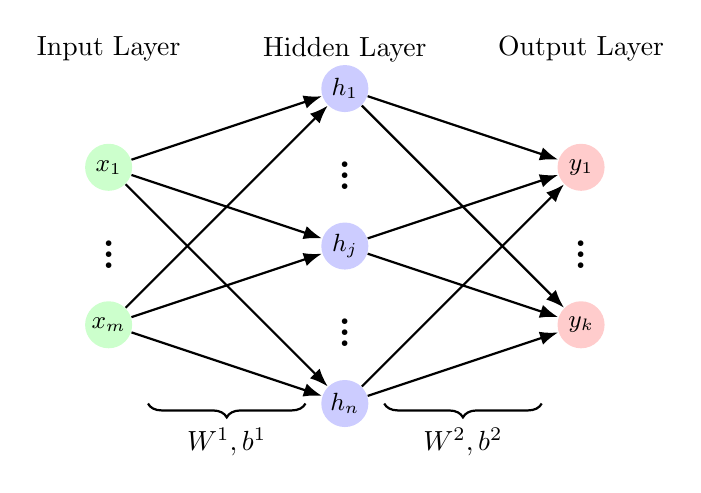
\begin{tikzpicture}[
        node distance=2cm, 
        neuron/.style={circle, fill=blue!20, minimum size=17pt, inner sep=0pt, font=\small},
        input/.style={neuron, fill=green!20},
        output/.style={neuron, fill=red!20},
        arrow/.style={-Latex, thick},
        dots/.style={font=\Huge, minimum height=1cm, inner sep=0, outer sep=0, node distance=0.5cm}
    ]
        % Input Layer
        \node[input] (I1) at (0, 2) {$x_1$};
        \node[input] (I2) at (0, 0) {$x_m$};
        \node[dots] (Idots) at (0, 1) {$\vdots$};

        % Hidden Layer
        \node[neuron] (H1) at (3, 3) {$h_1$};
        \node[neuron] (H2) at (3, 1) {$h_j$};
        \node[neuron] (H3) at (3, -1) {$h_n$};
        \node[dots] (Hdots) at (3, 2.0) {$\vdots$};
        \node[dots] (Hdots2) at (3, 0.0) {$\vdots$};

        % Output Layer
        \node[output] (O1) at (6, 2) {$y_1$};
        \node[output] (O2) at (6, 0.0) {$y_k$};
        \node[dots] (Odots) at (6, 1) {$\vdots$};

        % Arrows
        \draw[arrow] (I1) -- (H1); \draw[arrow] (I1) -- (H2); \draw[arrow] (I1) -- (H3);
        \draw[arrow] (I2) -- (H1); \draw[arrow] (I2) -- (H2); \draw[arrow] (I2) -- (H3);
        \draw[arrow] (H1) -- (O1); \draw[arrow] (H1) -- (O2);
        \draw[arrow] (H2) -- (O1); \draw[arrow] (H2) -- (O2);
        \draw[arrow] (H3) -- (O1); \draw[arrow] (H3) -- (O2);
        
        % Layer Labels
        \node at (0, 3.5) {Input Layer};
        \node at (3, 3.5) {Hidden Layer};
        \node at (6, 3.5) {Output Layer};
        
        % Braces
        \draw [decorate, decoration={brace, amplitude=5pt, mirror}, thick] (0.5, -1) -- (2.5, -1) node [midway, below=5pt] {$W^1, b^1$};
        \draw [decorate, decoration={brace, amplitude=5pt, mirror}, thick] (3.5, -1) -- (5.5, -1) node [midway, below=5pt] {$W^2, b^2$};

    \end{tikzpicture}
    } % End of \resizebox
    \caption{A simple Feed Forward Neural Network (FFNN) architecture with one input layer, one hidden layer, and one output layer. 
    Each neuron in a layer is connected to every neuron in the subsequent layer through weights ($W$) and biases ($b$).}
    \label{fig:ffnn-arch}
\end{figure}

\subsubsection{Prediction}

The process begins with the \textit{feed-forward pass}. For a given input vector $\boldsymbol{x}$, the activation $\boldsymbol{a}^l$ of layer $l$ is computed based on the activation of the previous layer $\boldsymbol{a}^{l-1}$ (where $\boldsymbol{a}^0 = \boldsymbol{x}$):

$$
\boldsymbol{z}^l = \boldsymbol{W}^l \boldsymbol{a}^{l-1} + \boldsymbol{b}^l
$$
$$
\boldsymbol{a}^l = f_l(\boldsymbol{z}^l)
$$
where $\boldsymbol{W}^l$ and $\boldsymbol{b}^l$ are the weight matrix and bias vector for layer $l$, and $f_l$ is the activation function. 
This process is repeated until the final output $\boldsymbol{a}^L = \hat{\boldsymbol{y}}$ is computed.

\subsubsection{Learning}

The network "learns" by minimizing a \textit{cost function} $\mathcal{C}(\boldsymbol{W}, \boldsymbol{b})$, which measures the discrepancy between the predicted output $\hat{\boldsymbol{y}}$ and the true target $\boldsymbol{y}$. 
This minimization is achieved using gradient-based optimization.

The \textit{backpropagation} algorithm is used to efficiently compute the gradient of the cost function with respect to every weight and bias in the network. 
It is an application of the chain rule, starting from the output layer and moving backward, here for a single training example:
\begin{enumerate}
    \item Compute the error $\boldsymbol{\delta}^L$ at the output layer $L$:
    $$ \boldsymbol{\delta}^L = \nabla_{\boldsymbol{a}^L} \mathcal{C} \odot f_L'(\boldsymbol{z}^L) $$
    \item Propagate the error backward to compute the error $\boldsymbol{\delta}^l$ for layer $l$:
    $$ \boldsymbol{\delta}^l = ((\boldsymbol{W}^{l+1})^T \boldsymbol{\delta}^{l+1}) \odot f_l'(\boldsymbol{z}^l) $$
    \item The gradient of the cost function with respect to the parameters of layer $l$ is then:
    $$ \nabla_{\boldsymbol{W}^l} \mathcal{C} = \boldsymbol{\delta}^l (\boldsymbol{a}^{l-1})^T $$
    $$ \nabla_{\boldsymbol{b}^l} \mathcal{C} = \boldsymbol{\delta}^l $$
\end{enumerate}
These gradients are then used by an optimization algorithm to update the weights and biases.



\subsubsection{Hyperparameters}
Just as with project 1, there are several hyperparameters to tune when setting up the FFNN, to get the best results.

\begin{itemize}
    \item \textbf{Learning Rate ($\eta$):} Controls how much to change the model in response to the estimated error each time the model weights are updated.
    \item \textbf{Number of Epochs:} The number of times the learning algorithm will work through the entire training dataset.
    \item \textbf{Batch Size:} The number of training examples utilized in one learning iteration.
    \item \textbf{Number of Hidden Layers and Units:} The architecture of the network, including how many hidden layers to use and how many neurons in each layer.
    \item \textbf{Activation Functions:} The choice of activation functions for each layer (e.g., ReLU, sigmoid, tanh).
\end{itemize}
In the results we will go through them to find a good approximation of the optimal parameters.
It is believed that deeper networks with more layers can capture more complex patterns, but they are also harder to train.

For more on FFNNs see chapter 1 and 2 in \cite[Nielsen]{NeuralNetworks}.

\subsection{Different Building Blocks}

\subsubsection{Cost Functions}

\textbf{Mean Squared Error (MSE)}
For regression tasks, we use the Mean Squared Error (MSE) cost function, which is identical to the one used in \cite{project1}. 
For a set of $n$ samples, it is:
$$
\mathcal{C}_{MSE}(\boldsymbol{W}, \boldsymbol{b}) = \frac{1}{n} \sum_{i=1}^n (y_i - \hat{y}_i)^2
$$
Its derivative with respect to a single final activation $\hat{y}_i$ (which is $a^L_i$) is computed as:
$$
\frac{\partial \mathcal{C}_i}{\partial \hat{y}_i} = 2(\hat{y}_i - y_i)
$$
where $\mathcal{C}_i = (y_i - \hat{y}_i)^2$ is the per-sample cost.

We extend this cost function to include $L_1$ and $L_2$ regularization, which helps prevent overfitting by penalizing large weights. 
The parameter $\lambda$ controls the strength of the regularization, see 3.4 \cite{hastie}.
\\

\textbf{L1 Regularization (LASSO):} 
The $L_1$ norm adds a penalty proportional to the absolute value of the weights, which encourages sparsity. This is the same technique used in LASSO regression in \cite{project1}. The cost function becomes:
$$
\mathcal{C}_{L1} = \mathcal{C}_{MSE} + \frac{\lambda}{2n} \sum_{l=1}^L \sum_{ij} |W^l_{ij}|
$$
The gradient of this term is:
$$
\nabla_{\boldsymbol{W}^l} \mathcal{C}_{L1} = \nabla_{\boldsymbol{W}^l} \mathcal{C}_{MSE} + \frac{\lambda}{2n} \cdot \text{sign}(\boldsymbol{W}^l)
$$

Where handling the non-differentiable L1 norm requires using a sub-gradient. For optimization, we use the sub-gradient of the penalty term, which is $\frac{\lambda}{2n} \cdot sign(W^{l})$, see 3.4.4 \cite{hastie}.
\\

\textbf{L2 Regularization (Ridge):} 
The $L_2$ norm adds a penalty proportional to the square of the weights. This is the same regularization technique used in Ridge regression in \cite{project1}. The cost function becomes:
$$
\mathcal{C}_{L2} = \mathcal{C}_{MSE} + \frac{\lambda}{2n} \sum_{l=1}^L \sum_{ij} (W^l_{ij})^2
$$
The gradient of this term, added during backpropagation, is:
$$
\nabla_{\boldsymbol{W}^l} \mathcal{C}_{L2} = \nabla_{\boldsymbol{W}^l} \mathcal{C}_{MSE} + \frac{\lambda}{n} \boldsymbol{W}^l
$$


\subsubsection{Activation Functions}
Disregarding the linear activation function used in the output layer for regression, we have three commonly used activation functions for the hidden layers of the network.
These are non-linear so that the FFNN model doesn't become the same as a network with zero hidden layers. 
i.e. matrices multiplied together is still a matrix.
\\

\textbf{Sigmoid}
An exponential function that has a range from 0 to 1, and a continues derivative.
A common problem with this method is diminishing gradients where the network will struggle to learn for large gradients. 
$$
\sigma(z) = \frac{1}{1+e^{-z}}
$$



\textbf{ReLU}
The Rectified Linear Unit (ReLU) is a piecewise linear function that outputs the input directly if it is positive; otherwise, it will output zero. This function has become the default activation function for many types of neural networks because a model that uses it can often converge faster than those using sigmoid or tanh functions.
$$
\text{ReLU}(z) = \max(0, z)
$$
\\

\textbf{Leaky ReLU}
The Leaky ReLU is a variant of the ReLU that allows a small, non-zero gradient $\alpha$ when the input is negative. 
This helps to mitigate the dying ReLU problem, where neurons can become inactive and stop learning entirely.
$$
\text{Leaky ReLU}(z) = \max(\alpha z, z)
$$

For more on activation functions see 14.12 in the lecture notes \cite{compfys}.

\subsubsection{Optimization Algorithms}
In a previous paper \cite{project1}, we implement three different gradient-based optimization algorithms to update the weights and biases of the gradient descent.
Where the most important where Stochastic Gradient Descent (SGD), RMSprop and Adam.
These methods are widely used in training neural networks due to their efficiency and effectiveness in handling large datasets (SGD) and adapting learning rates (RMSprop and Adam).
\\

\textbf{Stochastic Gradient Descent (SGD)} is an optimization method that approximates the full batch gradient by utilizing a small, randomly sampled subset of the data, known as a mini-batch $B_t$ of size $m$, at each iteration. 
This introduces stochastic noise into the optimization path. 
The update rule for SGD is the same as for standard gradient descent, but the gradient is computed over the mini-batch.
See 8.3.1 in \cite{Goodfellow} for more details.
\\

\textbf{RMSprop} is an optimization method designed to address the aggressively diminishing learning rates found in other adaptive methods like AdaGrad. 
It approximates a running average of the squared gradients by utilizing an exponentially decaying moving average, $E_t$, at each iteration. 
This helps prevent the learning rate from diminishing too quickly. 
The update rule for RMSprop scales the gradient by the inverse of this moving average: 
\begin{align*} 
    \theta_{t+1} &= \theta_t - \frac{\eta}{\sqrt{E_t + \epsilon}} \odot \nabla_{\theta} J(\theta_t) 
\end{align*} 
where $E_t$ is the moving average of the squared gradients and $\epsilon$ is a small smoothing constant. 
See 8.5.2 in \cite{Goodfellow}.
\\

\textbf{Adam} (Adaptive Moment Estimation) is an optimization method that combines the momentum method with the adaptive learning rate scaling of RMSprop. 
It maintains two exponentially decaying moving averages: a moving average of the gradients ($m_t$, the first moment) and a moving average of the squared gradients ($v_t$, the second moment). 
Adam is often considered a highly efficient and stable general-purpose optimizer. 
The update rules are:

\begin{align*} 
    m_{t+1} &= \beta_1 m_t + (1 - \beta_1) \nabla_{\theta} J(\theta_t) \\ 
    v_{t+1} &= \beta_2 v_t + (1 - \beta_2) (\nabla_{\theta} J(\theta_t))^2 \\ 
    \theta_{t+1} &= \theta_t - \frac{\eta}{\sqrt{v_{t+1} + \epsilon}} \odot m_{t+1} 
\end{align*} 
where $\beta_1$ and $\beta_2$ are decay rates for the moments and $\epsilon$ is a small smoothing constant. 
See 8.5.3 in \cite{Goodfellow}.
\\

The implementation of these methods for the FFNN followed a straightforward approach using the update rules or restrictions above. 
See the GitHub repository \cite{rep2} for the exact implementation.

\subsection{Image Classification}

When applying our FFNN model to an image classification task, one only needs to make a few adjustments to the architecture and cost function to suit the nature of classification problems.
Which we will then demonstrate on the MNIST dataset of handwritten digits.
This alternations to the architecture follow the book shown in \cite{NeuralNetworks} chapter 3.
\\

\subsubsection{Output layer}
For multiclass classification tasks, the output layer of the FFNN is modified to use the softmax activation function.
The softmax function converts the raw output scores (logits) from the final layer into probabilities for each class.
Given an input vector $\boldsymbol{z}$ from the final layer, the softmax function is defined as:
$$
\text{softmax}(z_i) = \frac{e^{z_i}}{\sum_{j} e^{z_j}}
$$
for each class $i$.
This ensures that the output probabilities sum to 1, making it suitable for multiclass classification tasks.
\\

\subsubsection{Cost Function}
For classification tasks, we replace the mean-squared error cost function with the cross-entropy loss function.
The cross-entropy loss measures the discrepancy between the predicted class probabilities and the true class labels.
For a single training example with true label $y$ (one-hot encoded) and predicted probabilities $\hat{\boldsymbol{y}}$, the cross-entropy loss is defined as:
$$
\mathcal{C}_{CE} = -\sum_{i} y_i \log(\hat{y}_i)
$$
where $y_i$ is 1 if the true class is $i$ and 0 otherwise.
This loss function encourages the model to assign high probabilities to the correct classes while penalizing incorrect predictions.
\\

\subsubsection{Learning}
These changes also affect the backpropagation process.
Where we now calculate the gradient of the cross-entropy loss with respect to the softmax outputs.
Lucky for us if we combine the softmax activation with the cross-entropy loss, the gradient simplifies to:
$$
\frac{\partial \mathcal{C}_{CE}}{\partial z_i} = \hat{y}_i - y_i
$$
This simplification makes the backpropagation process more efficient, as it avoids the need to compute the derivative of the softmax function separately.
For the exact derivation of this see \cite{mehta2023softmax}.

\subsection{Implementation and Code}
All code for this project was written in Python and is available in the GitHub repository \cite{rep2}.
Where we made use of the NumPy library for numerical computations \cite{numpy}, sklearn for machine learning utilities \cite{sklearn_api}, and Matplotlib for plotting results \cite{matplotlib}.
The implementation is organized into two main parts:
\begin{itemize}
    \item A Python file (Functions.py) containing the core NeuralNetwork class, all activation and cost functions, their derivatives, and optimization algorithms.
    \item Three Jupyter Notebooks used for running experiments, generating the results, and plotting the figures presented in this report.
\end{itemize}
\subsubsection{FFNN Implementation}

The FFNN was implemented from scratch using NumPy for all numerical computations. The core of the implementation is a NeuralNetwork class, which is designed to be modular and flexible. Upon initialization, it allows for easy adjustment of:
\begin{itemize}
    \item The number of layers and nodes per layer.
    \item The activation function for each layer (Sigmoid, ReLU, Leaky ReLU).
    \item The cost function (Mean Squared Error for regression, Cross-Entropy for classification).
    \item The optimization algorithm (SGD, RMSprop, ADAM).
    \item Regularization type (L1 or L2) and strength.
\end{itemize}
This modularity allows the same core class to be used for both regression and classification tasks by simply changing the cost function and final activation function.
\subsubsection{Testing and Comparison}
Before analyzing the model's performance, the correctness of the implementation was verified. 
The most critical component, the manually implemented backpropagation algorithm (compute gradient), was tested against automatic differentiation.
Using the autograd library, we computed the gradients numerically and compared them to our analytical gradients. 
As detailed in the Verification.ipynb notebook \cite{rep2}, the difference between the gradients was found to be on the order of $10^{-16}$ or lower, confirming that our backpropagation implementation is correct to a high degree of numerical precision.

Furthermore, a simple training run was conducted to verify that the cost function decreases over epochs and compared against the results from sklearn's MLPRegressor and our own implementation.
This discrepancy is likely due to differences in default hyperparameters that are non-trivial to align, but the model was still comparable to the scikit-learn implementation in performance on a dataset with $N=100$ samples.
I.e. there is no large discrepancy in performance that would indicate a faulty implementation.

The final results for the classification task was also compared to the literature on the MNIST dataset, where our results are in line with what is expected for a simple FFNN implementation, implying a correct implementation.

\subsection{Use of AI tools}
While writing and correcting the code for this project github copilot was used to help with some of the boilerplate code and finding bugs.
For writing the report Gemini 2.5 was used as an editor to help with structuring sentences and paragraphs. 
Though this editing was only done at the end of writing the complete structure of the report, to avoid any influence on the content itself. 


\section{Results and Discussion}\label{section:results}
Before presenting the results, it is important to note the evaluation methodology used. 
For all regression experiments, we select the best model from all iterations based on its lowest achieved test MSE score during training. 
While this is a standard approach for model selection, we will later discuss the potential risks of this method when applied to a very sparse dataset.

\subsection{Training the FFNN for Regression}
To begin our exploration of the FFNN's capabilities in regression, we first established a performance baseline with a "naive" model. This configuration used simple gradient descent, a fixed learning rate of $\eta=0.1$, and the Sigmoid activation function.

\begin{figure}[htbp]
    \centering
    \includegraphics[width=\columnwidth]{figures/MSE_Heatmap_Layers_Nodes.png}
    \caption{Heatmap showing that the FFNN without any optimizations is struggling to learn anything useful after 1000 epochs of training.}
    \label{fig:figure1}
\end{figure}

The results, shown in Figure \ref{fig:figure1}, demonstrate that this simple configuration fails to learn the underlying Runge function. 
The test MSE remains high across all tested architectures, with the best-performing (and simplest) model only achieving a score that is not significantly better than the others.  

This failure is characteristic of the well-known vanishing gradient problem.
The Sigmoid activation function's saturated outputs stop the flow of gradients to earlier layers, effectively halting the learning process. 
This hypothesis was confirmed by a longer training run (Figure \ref{fig:long-training}) on a more complex architecture, which revealed that the training score did not begin to decrease until approximately 10,000 epochs, demonstrating an extremely inefficient learning process.
\begin{figure}
    \centering
    \includegraphics[width=\columnwidth]{figures/Learning_Curve_2Layers_50Nodes.png}
    \caption{Training and test MSE over 20000 epochs for a FFNN with 2 hidden layers and 50 nodes per layer using plain gradient descent with a learning rate of 0.1 and sigmoid activation function.}
    \label{fig:long-training}
\end{figure}

The baseline failure highlights the necessity of modern components to overcome these training challenges. 
We first investigated the impact of replacing gradient descent with adaptive optimization algorithms: Stochastic Gradient Descent (SGD), Adam, and RMSprop.

\begin{figure}[htbp]
    \centering
    \includegraphics[width=\columnwidth]{figures/OptimizationsAreImportant.png}
    \caption{Heatmap showing that the choice of optimization algorithm has a significant impact on the FFNN's performance in learning.}
    \label{fig:optimization-importance}
\end{figure}

As seen in Figure \ref{fig:optimization-importance}, this choice has a dramatic impact. Both RMSprop and Adam, which utilize adaptive learning rates, achieve significantly lower MSE scores than standard GD or mini-batch SGD. RMSprop, in particular, appears to be the most effective for this task.  

To isolate the impact of the adaptive algorithm itself from the use of mini-batches, we can compare standard GD against mini-batch SGD. Both methods performed equally poorly, confirming that the superior performance of RMSprop and Adam is not merely due to more frequent updates, but stems directly from their advanced adaptive learning rate mechanisms.  

Having established the necessity of an adaptive optimizer, we then investigated the interaction between activation functions and learning rates.

\begin{figure}[htbp]
    \centering
    \includegraphics[width=\columnwidth]{figures/MSE for Different Activation Functions.png}
    \caption{Heatmap showing that change in one hyperparameter can imply a change in the optimal value of another hyperparameter.}
    \label{fig:freezing-problems}
\end{figure}

Figure \ref{fig:freezing-problems} reveals two key findings. 
First, the Sigmoid function consistently underperforms regardless of the learning rate, reinforcing its unsuitability. 
Second, it illustrates a strong interaction effect: the optimal learning rate is clearly dependent on the chosen activation function. 
Leaky ReLU, for instance, achieves its best performance at $\eta=0.01$, while sigmoid performs best at $\eta=0.1$.
 
This analysis also highlights the complex interplay between hyperparameters, motivating a more comprehensive grid search to identify optimal configurations.

\subsection{A deceptive search tuning and regularization on sparse data}
The analysis in above established that a functional model requires an adaptive optimizer.
The next logical step is to determine the optimal network architecture and, crucially, the correct regularization strategy to prevent overfitting on our sparse dataset.

To find these parameters, we performed a comprehensive, cross-validated grid search over the learning rate, number of layers, nodes per layer, and activation function. The methodology is detailed in the GridSearch.ipynb notebook.

However, it is critical to address the primary challenge of this regression task, the sparse dataset ($N=18$).  
Our methodology of selecting the model with the lowest test MSE during training carries a significant risk of overfitting to the test set. 
The model may learn to fit the specific noise of the 4 test points, not the true underlying function.

Therefore, to obtain a true, unbiased measure of generalization, we adopted a two-stage evaluation:
\begin{enumerate}
    \item First, use the cross-validated grid search on our "known" dataset to find our contender for the best hyperparameters for the unregularized (L0), L1-regularized, and L2-regularized models.
    \item Second, compare the generalization performance of these three "best" models on a new, unseen dataset of 100 data points to see how well they generalize to the actual function.
\end{enumerate}

\subsubsection{No Regularization}
The best unregularized model, table \ref{tab:hyperparameters_l0}, achieved a final test MSE of -2.834 on the original sparse test set.
This test score is significantly higher than the best analytical OLS solution from our previous work (-1.997).


\begin{table}[htbp]
    \caption{Best hyperparameters found for the FFNN regression task without regularization}
    \label{tab:hyperparameters}
    \begin{ruledtabular} % This replaces \centering and adds the lines
    \begin{tabular}{l r}
        % No \hline\hline needed - ruledtabular does it.
        \textbf{Parameter} & \textbf{Value} \\
        \colrule % This is the revtex4 replacement for \midrule or \hline
        Hidden layers & 2 \\
        Nodes per layer & 10 \\
        Activation function & LeakyReLU \\
        Learning rate & 0.1 \\
        Batch size & 5 \\
        Optimizer & RMSprop \\
        \colrule
        \textbf{Final Cost} & \textbf{-2.834}
    \end{tabular}
    \end{ruledtabular}
\end{table}

However, the fit in figure \ref{fig:ffnn-no-regularization}, shows that the chosen function has fitted to the test points rather than the necessarily the training points.
Showing that this naive search for the optimal parameters has overfitted to the test set.
We will later see that this overfitting does not translate to poorer generalization on new data, but it is a clear fault in our selection methodology on sparse data.

\begin{figure}[htbp]
    \centering
    \includegraphics[width=\columnwidth]{figures/ffnn_fit_plot_L0.png}
    \caption{FFNN regression results without regularization on noisy data.}
    \label{fig:ffnn-no-regularization}
\end{figure}


\subsubsection{$L1$ Regularization}
Echoing the same sentiment as earlier we did a grid search over several hyperparameters to find the best combination for the FFNN with $L1$ regularization.
The best result for the regularization $L1$ with a noisy dataset was:
\begin{table}[htbp]
    \caption{Hyperparameters used for the neural network with $L1$ regularization}
    \label{tab:hyperparameters}
    \begin{ruledtabular} % This replaces \centering and adds the lines
    \begin{tabular}{l r}
        % No \hline\hline needed - ruledtabular does it.
        \textbf{Parameter} & \textbf{Value} \\
        \colrule % This is the revtex4 replacement for \midrule or \hline
        Hidden layers & 2 \\
        Nodes per layer & 20 \\
        Activation function & LeakyReLU \\
        Learning rate & 0.1 \\
        Batch size & 10 \\
        Optimizer & RMSprop \\
        Regularization($\lambda$) & 1e-05 \\
        \colrule
        \textbf{Final Cost} & \textbf{-2.934}
        % No \bottomrule or \hline\hline needed
    \end{tabular}
    \end{ruledtabular}
\end{table}

Which was found after 79 epochs of training.
If we compare this to what we found in the previous project \cite{project1} of -2.10 for the lasso regression after training for 9998 epochs.
We see that the FFNN is able to outperform the Lasso solution here as well.


\begin{figure}[htbp]
    \centering
    \includegraphics[width=\columnwidth]{figures/ffnn_fit_plot_L1.png}
    \caption{FFNN regression results with L1 regularization on noisy data.}
    \label{fig:ffnn-l1-regularization}
\end{figure}

Where we find the same trend as with the previous results \cite{project1}, that since the data is so sparse the model doesn't benefit much from the regularization.
Or at least not in a way that is visible from the test cost on new data.

\subsubsection{$L2$ Regularization}

Best result for the regularization $L2$ with a noisy dataset:
\begin{table}[htbp]
    \caption{Hyperparameters used for the neural network with $L2$ regularization}
    \label{tab:hyperparameters}
    \begin{ruledtabular} % This replaces \centering and adds the lines
    \begin{tabular}{l r}
        % No \hline\hline needed - ruledtabular does it.
        \textbf{Parameter} & \textbf{Value} \\
        \colrule % This is the revtex4 replacement for \midrule or \hline
        Hidden layers & 2 \\
        Nodes per layer & 10 \\
        Activation function & LeakyReLU \\
        Learning rate & 0.1 \\
        Batch size & 3 \\
        Optimizer & RMSprop \\
        Regularization($\lambda$) & 2e-04 \\
        \colrule
        \textbf{Final Cost} & \textbf{-2.491}
        % No \bottomrule or \hline\hline needed
    \end{tabular}
    \end{ruledtabular}
\end{table}

Based on this search, one would conclude that the L1 model is the best. 
But given the clear overfitting in Figure \ref{fig:ffnn-no-regularization}, and the sparse test data, these scores are unreliable.

\subsubsection{Final Comparison regression}
The limitations of the sparse-set search are fully exposed when we evaluate these three best models on the new, 100-point dataset. 
This provides an unbiased measure of their true generalization.

\begin{figure}
    \centering
    \includegraphics[width=\columnwidth]{figures/Comparison of Models on 100 Extra Data Points.png}
    \caption{Final comparison of the three FFNN regression models on new data.}
    \label{fig:final-comparison-regression}
\end{figure}

The results of this benchmark figure \ref{fig:final-comparison} reveal the real story. 
Where The L1-regularized FFNN is the clear winner, achieving the best generalization score of all models -1.82. 
It outperforms not only the other FFNNs but also all analytical methods from our previous study.

The unregularized model, which scored an impressive -2.834 on the sparse set, generalizes poorly with a score of -1.715. 
This confirms that some regularization is indeed necessary to prevent overfitting, even if the sparse-set search failed to reveal this.
One should use some amount of regularization to have a more generalizable model, which is especially pronounced problem in sparse datasets.

This benchmark provides a key insight into why the L1-regularized model won. 
The task involves an over-parameterized model (a 2-layer FFNN with hundreds of parameters) fitting a simple 1D function from extremely sparse data.  
L2 (Ridge) regularization shrinks all weights but keeps them non-zero, resulting in a complex, "dampened" function.   
L1 (Lasso), by contrast, induces sparsity by "pruning" weights, forcing many to zero. 
This performs a type of automatic model selection, simplifying the network.  

For this specific problem, L1's aggressive simplification created a less complex model that was less prone to fitting noise and therefore generalized far better. 
The danger was not just in overfitting, but in trusting a validation metric that was, itself, overfitted.


\subsection{Image Classification}
Now we will use the methods we learned from the regression task to implement a FFNN for image classification on the MNIST dataset.
Especially the knowledge gleamed around overfitting, the need for regularization and that slow and steady learning is better than fast and unstable learning.

To solve this, we will adapt the output layer to use the softmax activation function and the cross-entropy cost function.
Where we in this case will have alot more data to train on and therefore escape the randomness contained in comparing sparse data sets.  

As we experience before finetuning the hyper parameters one by one does not create a network of complex results where the relationship between the two show the full picture of how they interact with each other.
I.e. we will try on this larger set to se if our grid search can find some good suggestions for the best hyper parameters for the MNIST dataset.

As the MNIST dataset is much larger than the sparse dataset we had for the regression task, we need to use a smaller grid search, fewer epochs.
We are also not able to use the whole training dataset for each training run as it would be too computationally expensive.
Therefore we use a subset of 1000 samples from the training set for each training run.
After running this code for a while we found a suggestion for what the optimal parameters where when trained for 5 epochs on each combination.


Looking at the results that our naive grid search found and then training it for longer on these parameters. 
We saw that we are optimizing for the parameters that give us the best results after 5 epochs, was a good starting point.
Where we could then tune it further, by doing an educated guess that to use a lower learning rate and a larger batch size will improve the stability in learning.
After having gone through this process a few times we found a good set of hyperparameters that gave us good results on the MNIST dataset.

\begin{table}[H]
    \caption{Hyperparameters used for the neural network training.}
    \label{tab:hyperparameters}
    \begin{ruledtabular} % This replaces \centering and adds the lines
    \begin{tabular}{l r}
        % No \hline\hline needed - ruledtabular does it.
        \textbf{Parameter} & \textbf{Value} \\
        \colrule % This is the revtex4 replacement for \midrule or \hline
        Learning rate & 0.001 \\
        Batch size & 64 \\
        Hidden layers & 3 \\
        Nodes per layer & 100 \\
        Activation function & sigmoid \\
        Optimizer & RMSprop \\
        Regularization Type & L2 \\
        Regularization($\lambda$) & 1e-03 \\
        \colrule
        \textbf{Final Accuracy} & \textbf{97.51\%} \\
        % No \bottomrule or \hline\hline needed
    \end{tabular}
    \end{ruledtabular}
\end{table}

As the final results was a bit off from our new findings, this implies the need for a better hyperparameter tuning method, one that perhaps tunes for training runs that has a consistent and steady improvement rather than finding the lowest cost after a few epochs, as running on the whole dataset for many epochs is computationally infeasible in practice.
Even for this small set of hyperparameters it took a long time to run through all the combinations.

\begin{figure}[htbp]
    \centering
    \includegraphics[width=\columnwidth]{figures/MNIST_Learning_Curve.png}
    \caption{The training and test accuracy and loss for our MNIST classification model}
    \label{fig:mnist-accuracy-loss}
\end{figure}

Analyzing our training curve in fig. \ref{fig:mnist-accuracy-loss} we see that the model is learning quite well and is not beginning to overfit before after 17 epochs.
Where we see that the training accuracy is still decreasing while the test accuracy begins to increase.

If we now want to look at how the model is actually performing on this test set we can look at the confusion matrix in fig. \ref{fig:mnist-confusion-matrix}.
Where we see that the model is performing quite well, with a high percentage of the predictions being on the diagonal, i.e. correctly classified.

\begin{figure}[htbp]
    \centering
    \includegraphics[width=\columnwidth]{figures/MNIST_Confusion_Matrix.png}
    \caption{Heatmap of the confusion matrix for our MNIST classification model}
    \label{fig:mnist-confusion-matrix}
\end{figure}

We see that the mistakes of classifying 5 as a 3 is the most common mistake, which is interesting as they don't look that similar.
We believe that this is in some part due to the way people write these digits and that the FFNN isn't necessarily trained to capture the same features as we look for.
It might learn this through its neurons but it might also learn to classify it in other ways, e.g. the explainability of a prediction is what makes it hard to pinpoint why.

\begin{figure}
    \centering
    \includegraphics[width=\columnwidth]{figures/misclassified_5_as_3.png}
    \caption{Misclassified 5 as 3 from the MNIST test set}
    \label{fig:mnist-misclassified-examples}
\end{figure}
Looking closer at  some of these mistakes in fig. \ref{fig:mnist-misclassified-examples} we see that there should be some room for improvement here.
As all of these looks like 5s, perhaps the middle one can be seen as a 3, so a neural network that is better at capturing spatial hierarchies might help.
In view of this there should be possible to make some more improvements to this classification. 
Perhaps by using a convolutional neural network (CNN) that is better suited for image data, as it can capture spatial hierarchies in images better than a FFNN.


As a concluding remark we see that the FFNN model is able to perform quite well on the MNIST dataset out of the box in achieving an accuracy of 97.51\%.
Where it has shown clear capabilities and adaptability to learn complex functions from data.


\section{further work}
Some ideas for further work:
\begin{enumerate}[a)]
    \item Research on finding more cost efficient ways to do hyper parameter tuning.As the naive approach we used is very computationally expensive.There should be some clever way to do this that doesn't require as many training runs and uses statistics to find the best parameters faster.
    \item How different architectures with regards to layers and nodes per layer affect the learning capabilities of the FFNN. Are triangles better than rectangles? Is it better to have one hidden activation function for all layers or to mix them? 
    \item How parallelization and GPU acceleration can speed up the training process for FFNNs implemented from scratch.
\end{enumerate}






\section{Conclusion}\label{section:conclusion} 
Just as with the analytical methods from \cite{project1} we found that working on a sparse dataset made it hard to see the benefits of regularization, even with the added noise.
However, we still found that the FFNN was able to outperform the analytical methods in both the unregularized and regularized cases.
Showing the power of neural networks in adapting to complex functions.

Though the real problem grasped from this project is the hyperparameter tuning.
Where we found that the naive approach of freezing all but two hyperparameters and then plotting a heatmap to find the best combination was flawed.
While doing an exhaustive grid search was computationally expensive and still didn't guarantee the best results.
As we where measuring it along a few epochs and chose the one that had the best run out of these few epochs.
A better approach would perhaps be to see how steady the improvement was over time rather than just looking at the best result after a few epochs.

We also found that the choice of optimization algorithm had a significant impact on the learning capabilities of the FFNN.
Where Adam and RMSprop was needed in order to get good results, as plain SGD struggled to learn anything useful.

For specifically sparse datasets we found that when tuning the hyperparameters one will have a continuous struggle to find the best combination for the underlying dataset as each epoch will have a randomness where it might just inch closer to the test set and away from the training set.

When it comes to the image classification task we found that the FFNN was able to perform quite well on the MNIST dataset, achieving an accuracy of 97.51\%.
However, if we compare this to the performance of the best solutions to this problem we find that there is still much room for improvement as state-of-the-art models achieve accuracies above 99.7\%.
Which is even higher than what human performance on this task is believed to be within.

\bibliography{biblio}

% \appendix with table of hyperparameters and values for the models
\end{document}
